\section{Щелочные металлы и их соединения в технике и технологии. Щелочноземельные
металлы и их соединения в современных материалах.} % каждый section это 1 билет. Если нужны подразделы, то \paragraph{}
\underline{\textbf{Щелочные металлы:}}
\par 1) Na-K эвтектика (теплоносители в АЭС)
\par 2) регенерация воздуха на подлодках: $\rm 4KO_2 + 2CO_2 = 2 K_2CO_3 + 3O_2 \uparrow$
\par 3) натриевые лампы (газовый разряд в парах Na)
\par 4) Топливо в термоядерной бомбе: \par $\rm {}_6^3Li + {}_0^1n \rightarrow {}_1^3H+{}_2^4He$ \par ${}_1^3H + {}_1^2H \rightarrow {}_2^4He + {}_0^1n$
\par 5) калийные удобрения ($\rm KNO_3$)
\par 6) физраствор NaCl
\par 7) цезиевые фотоэлементы
\par 8) магнитогидродинамический генератор на цезиевой плазме (струя холодной 1000 К плазмы гонится по трубе в мощном поперечном магнитном поле, сила Лоренца раскидывает разноимённые заряды к разным сторонам трубы, мы снимаем напряжение)
\par 9) стёкла ($\rm Na_2O\cdot CaO \cdot 6SiO_2$ - оконное, $+SiO_2$ - пирекс)
\par10) Na-ионные батареи
\par
\underline{\textbf{Щелочноземельные металлы:}}
\par \underline{Be}: в 1,5 раза легче Al $\Rightarrow$ беррилиевые моторы для F-1
\par - бериллиевые бронзы (Cu+2-3\% Be) - лёгкость, износоустойчивость, упругость
\par - окна для рентгеновских трубок (слабо поглощает рентген)
\par -  замедлитель нейтронов
\par - покрытия космических кораблей, беррилизация стали (10-15 часов при 1000 $^\circ$ C в порошке бериллия)
\par -  $\rm Be_2O3$ - хорошо проводит тепло, при этом огнеупор.
\par \underline{Mg}:
\par - лёгкие сплавы
\par - зажигательные снаряды, трассирующие пули, осветительные ракеты
\par - слабительное $\rm MgSO_4\cdot 7H_2O$
\par - реактивы Гриньяра, металлотермия (получение Ti, V, Cr, Zr)
\par - магнезиальный цемент (цемент Сорреля): $\rm MgCl_2 + MgO$
\par бактерицидные, фунгицидные свойства, огнеупор, маслостойкость, солестойкость
\par \underline{Ca}:
\par - гипс $CaSO_4\cdot 2 H_2O$
\par - $\rm CaCl_2$ - осушитель
\par - восстановитель
\par - геттер в вакуумной технике
\par - стёкла (CaO)
\par - цементы (CaO)
\par - $\rm {}_{20}^{48}Ca$ для синтеза трансурановых элементов
\par \underline{Sr}: 
\par - пиротехника (ярко-красный)
\par - $\rm {}^{90}Sr$ - бета-излучатель
\par - SrO хорошо поглощает рентгеновское излучение (добавка к стёклам старых телевизоров для защиты от излучения кинескопов)
\par \underline{Ba}:
\par - $\rm BaSO_4 $ - поглотитель рентгеновских лучей (медицина)
\par - пиротехника (жёлто-зелёный)
\par - $\rm BaTiO_3$ - сегнетоэлектрик
\par - ВТСП-керамика
\section{Бор, алюминий, галлий, индий, таллий и их соединения в современной
технике и технологии.}
\underline{B}:
\par - борная кислота $\rm B(OH)_3$ - дезинфекция
\par - $\rm Na_2B_4O_7$ - восстановитель, удобрения
\par - $\rm B_4C$  - абразивы, бронежилеты, поглотитель нейтронов
\par - BN - абразив
\par - $\rm BF_3$ - катализатор в органическом синтезе (ядовит!)
\par \underline{Al}:
\par - фольга
\par - лёгкие сплавы (дюраль, силумин, авиаль)
\par - провода (трескаются, ибо металл хрупкий)
\par - керамические материалы, ювелирные изделия (шпинель $\rm MgAl_2O4$)
\par - сапфировые монокристаллические подложки
\par - катализатор Фриделя-Крафтса ($\rm AlCl_3$)
\par - активный восстановитель
\par - анодированный алюминий для неорганических мембран, 1D-структур, катализаторов, корпусных материалов
\par \underline{Ga}:
\par - полупроводники $\rm A^{III}B^{V}$
\par - сплавы с Bi, Pb, Sn, Cd в термопредохранителях
\par - высокотемпературные термометры ($T_\text{пл}<100^\circ C$)
\par - покрытия для высокоотражающих зеркал
\par - легкоплавкие сплавы в термометрах вместо ртути (галинстан, $T_\text{пл}=-19,5^\circ C$)
\par - теплоноситель в АЭС
\par - материал для создания ионных пучков
\par \underline{In}:
\par - полупроводники $\rm A^{III}B^{V}$
\par - антифрикционные покрытия
\par - поглотитель нейтронов
\par - покрытия для высокоотражающих зеркал
\par - ITO (In Sn O) - прозрачный проводник
\par - легкоплавкий припой с высокой адгезией
\par \underline{Tl}: крайне токсичен!
\par - полупроводники $\rm A^{III}B^{V}$
\par - галогениды таллия - линзы в ИК-диапазоне
\par - низкотемпературные термометры (Tl+Hg: $T_\text{пл}=-61^\circ C$)
\par - ВТСП
\par - активатор в стинцилляторах на основе NaI
\section{Материалы на основе d- и f- элементов. Материалы на основе 3d-элементов}
5f-элементы все радиоактивны. Большое практическое применение у $\rm {}^{238}U$ (атомное топливо) и Pu (оружейный). \par
4f-элементы используются в люминесцентных материалах, магнитах, катализе (Ce), лазерных материалах
\par На  основе d-металлов изготавливают магнитные материалы, катализаторы (Rh-Au), жаропрочные сплавы (W), высокопрочную керамику ($\rm ZrO_2$), топливные элементы, легированные стали
\par \underline{\textbf{3d}}
\par \underline{Sc}: сплавы, высокотвёрдые материалы (легирование WC), рентгеновские зеркала $\rm Sc_2O_3$ - жаростойкая прочная керамика, добавка в ртутные лампы, чтобы спектр был ближе к солнечному
\par \underline{Ti}: импланты, корпуса подлодок, геттер в вакуумной технике, нитинол (Ni+Ti), легированные стали, TiN (покрытия), $\rm TiO_2$ (фотокатализатор, УФ-фильтр, белый пигмент), ячейки Гретцеля. Обладает рекордными значениями удельной прочности, коррозионно стоек, биосовместим.
\par \underline{V}: прочные стали для военной техники, раскислитель сталей, катализатор окисления $\rm SO_2$, катодные материалы для Li-ion (ванадаты). Ядовит!
\par \underline{Cr}: легирование сталей (нержавейка, 13 \% Cr), сплавы (хромель, нихром, фехраль), антикоррозионные покрытия, материалы для лопаток газовых турбин, $\rm Cr_2O_3$ - зелёный пигмент, абразив, катализатор. $\rm FeCr_2O_4$ - хрупкий огнеупор, $\rm LaCrO3$ - высокоточные нагреватели
\par \underline{Mn}: легированные стали, манганин (слабая зависимость сопротивления от Т, материал для реостатов). $\rm MnO_2$ - окислитель ("гопкалитовые патроны"), $\rm KMnO_4$ - окислитель. $\rm LiMn_2O_4$ - катоды в Li-ion. Сталь Гатфилда (танковые гусеницы).
\par \underline{Fe}: стали, чугуны, коричневый пигмент ($\rm Fe_2O_3$), магнитные материалы (ферриты)
\par \underline{Co}: коррозионностойкие сплавы, $\gamma$-нож (${}^{60}Co$),  ${}^{57}Co$ в Мёссбауэровской спектроскопии, синие пигменты, катоды в Li-ion, производство витамина B12
\par \underline{Ni}: монетные сплавы, тонкие защитные покрытия, металл-гидридные аккумуляторы, катализ, сплавы: мельхиор, нихром, пермаллой (сплав с нулевой магнетострикцией, для трансформаторных пластин), инвар (не удлиняется при нагреве), монель-металл. 
\par \underline{Cu}: провода, сплавы (латунь, бронза, монетные сплавы), ювелирные изделия, фунгицид $\rm CuSO_4$, поделочный камень малахит ($\rm Cu_2(OH)_2CO_3$), CuO для окраски стекла,ВТСП, полупроводник - $\rm Cu_2O$.
\par \underline{Zn}: защитные покрытия, латунь, ZnO - белый пигмент, фотокатализатор, полупроводники $\rm ZnB^{VI}$
\section{Точечные дефекты, квазихимическая модель. Дислокации (векторное и
континуальное описание). Вектор Бюргерса. Упругая энергия и плотность
дислокаций}
\underline{Точечный дефект} - локальное нарушение порядка в кристалле (отсутствие атома в узле решётки, атом в междоузлии, инородный атом в узле решётки). Выделяют точечные дефекты по Френкелю (атом из узла смещён в междоузлие с образованием пары "вакансия + атом в междоузлии) и по Шоттки (атом из узла удалён из кристалла, образовалась вакансия). В рамках квазихимической модели считается, что точечные дефекты образуют идеальный раствор в объёме кристалла (строго говоря, это не так, на самом деле дефекты взаимодействуют). \par
\underline{Обозначения по Крёгеру-Винку:} $V_M^X,V_X^X$ - незаряженная вакансия; $M_i^{\cdot}, X_i^{'}$ - катион/анион в междоузлии; $e^{'}$ - электрон, $h^{\cdot}$ - дырка. \par
С использованием этих обозначений записываются квазихимические уравнения, с помощью которых можно описывать процессы в твёрдом теле, зная константы соответствующих равновесий.
\par
Доминирующий тип дефектов (Шоттки/Френкель) определяется структурой кристалла, соотношением размеров катиона и аниона. Точечные дефекты формируют в материале быстро затухающие поля напряжений и деформаций $\sigma, \varepsilon \sim \frac{1}{r^3}$. \par
\underline{Дислокация} - протяжённый дефект, представляющий собой нарушение упорядоченного расположения атомных плоскостей в кристалле. Представить дислокацию удобно при помощи континуального описания (т.н. дислокации Вольтерра, (рис. \ref{fig:volterra_dislocation})
\begin{figure}[h!]
\centering
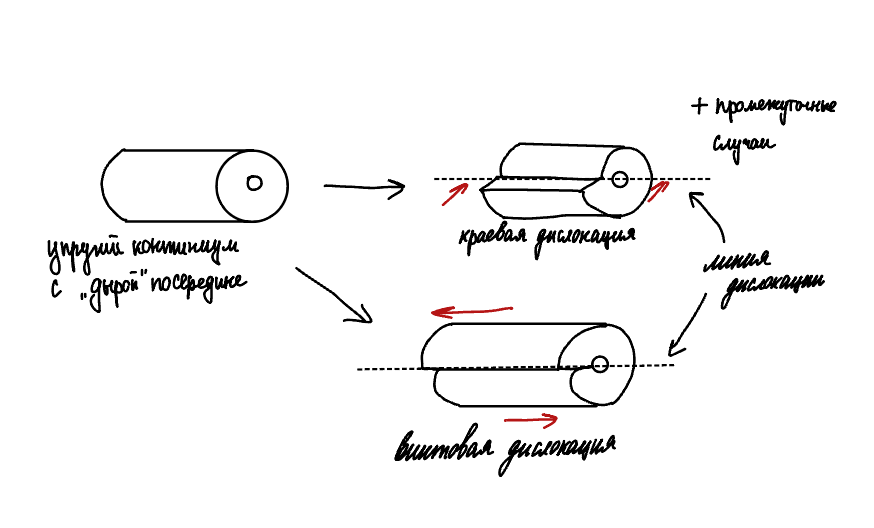
\includegraphics[width=0.55\textwidth]{volterra_dislocation.png}\caption{Дислокации Вольтерра} \label{fig:volterra_dislocation}
\end{figure} 
Сдвигом упругого континуума к оси цилиндра мы получаем краевую дислокацию, а сдвигом вдоль оси цилиндра - винтовую. Возможны и смешанные варианты.\par
Краевая дислокация представляет собой внедрение дополнительной атомной плоскости в кристалл (рис. \ref{fig:edge_dislocation}). Вдоль линии дислокации разупорядочение структуры максимально.
\begin{figure}[h!]
\centering
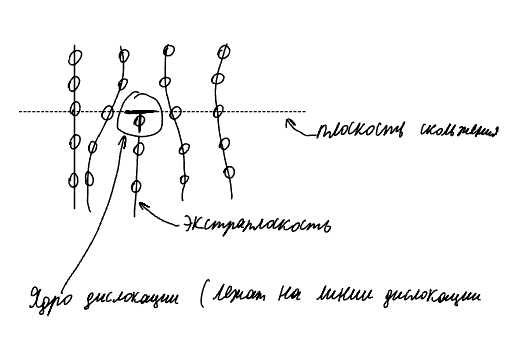
\includegraphics[width=0.55\textwidth]{edge_dislocation.png}\caption{Краевая дислокация}\label{fig:edge_dislocation}
\end{figure} 
\par
Дислокации удобно описывать при помощи вектора Бюргерса $\vec{b}$. Это вектор невязки между завершённым контуром в идеальном кристалле и аналогичным ему завершённым контуром, захватывающим дислокацию в реальном кристалле (рис. {\ref{fig:Burgers_vector}}).
\begin{figure}[h!]
\centering
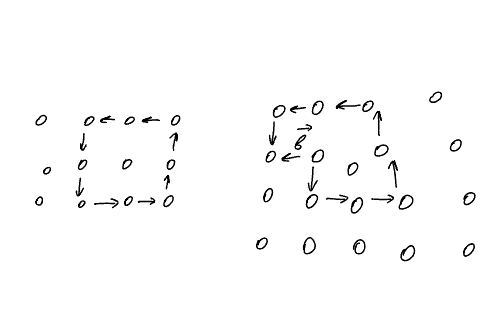
\includegraphics[width=0.55\textwidth]{Burgers_vector.png}\caption{К определению вектора Бюргерса} \label{fig:Burgers_vector}
\end{figure} 
\par
Краевая дислокация: $\vec{b}\perp$ линии дислокации\par
Винтовая дислокация: $\vec{b}\parallel$ линии дислокации\par
Вдоль линии дислокации $\vec{b}=const\Rightarrow$ дислокация не может оборваться внутри кристалла, должна либо замкнуться, либо расщепиться, либо выйти на поверхность.\par
Дислокации существенным образом искажают решётку, вызывая значительное поле напряжений и деформаций. Для винтовой дислокации 
\begin{equation}
    \varepsilon \sim \frac{b}{2\pi r}, \sigma \sim \frac{Gb}{2\pi r}
\label{eq:dislocation_force_field} %так как все билеты в последствии будут собираться в book, то картинки и ссылки должны называться осмысленно 
\end{equation}
В случае краевой дислокации возникает зависимость $\varepsilon$ и $\sigma$ от угла, хотя в целом $\varepsilon, \sigma \sim \frac{1}{r}$, то есть, поле затухает медленно.
\begin{equation}
   E_{\text{дислокации}}=E_{\text{ядра}}+E_{\text{упр}}
\label{eq:dislocation_energetics} 
\end{equation}
\begin{equation}
   E_{\text{упр}}=\frac{Gb^2}{4\pi}\ln \frac{r}{r_0} \text{ для винтовой дислокации}
\label{eq:screw_dislocation_energetics} 
\end{equation}
\begin{equation}
   E_{\text{упр}}=\frac{Gb^2}{4\pi(1-\nu)}\ln \frac{r}{r_0} \text{ для краевой дислокации}
\label{eq:edge_dislocation_energetics} 
\end{equation}
Здесь $\nu$ - коэффициент Пуассона, $r_0$ - размер ядра дислокации ($r_0 \sim 5-10 b$). \par
Плотность дислокаций определяется выражением \ref{eq:density_dislocation}:
\begin{equation}
   \rho=\frac{l}{V}
\label{eq:density_dislocation} 
\end{equation}
Здесь $l$ - полная длина дислокаций в образце объёмом $V$. В хорошо отожжённых металлах $\rho \sim 10^6-10^8$ см$^{-2}$. В полупроводниках $\rho \sim 10-10^5$ см$^{-2}$. После пластической деформации металла плотность дислокаций может достигать $\rho \sim 10^12-10^14$ см$^{-2}$. Для определения $\rho$ можно протравить шлиф, определить число ямок травимости - это точки выхода дислокаций на поверхность - и посчитать $\rho=\frac{N}{S}$.
\section{Плоское скопление дислокаций. Дефекты упаковки, двойниковые дефекты.
Оценка энергии дефекта упаковки по ширине растянутой дислокации}
\underline{Плоское скопление дислокаций} - это структура, представляющая собой n дислокаций, расположенных в одной плоскости скольжения перед дефектом, тормозящим скольжение дислокаций (напр. - граница зерна). Математическое описание такой структуры составляет суть задачи Набарро-Херринга. Можно получить, что положениям дислокаций в плоском скоплении соответствуют нули полинома Лагера. 
\begin{figure}[h!]
\centering
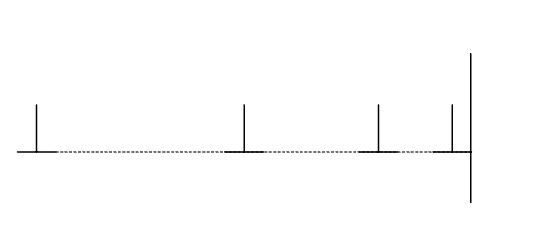
\includegraphics[width=0.55\textwidth]{dislocation_pile.png}\caption{Плоское скопление дислокаций}\label{fig:dislocation_pile}
\end{figure} 
\par Эта структура возникает вследствие отталкивания дислокаций одного знака. В головном скоплении на дислокацию действует сила $F=nF_d=n\tau b$, где $\tau$ - внешнее касательное напряжение, $b$ - вектор Бюргерса, $F_d$ - сила по формуле Мотта. \par
Это означает, что с ростом числа дислокаций существенно возрастает напряжение на границе зерна, так что при некотором значении $\tau$ дислокации начнут проскакивать через границу $\Rightarrow$ наблюдаем предел текучести на кривой нагружения. \par 
Можно получить, что число дислокаций $n\sim D \tau$, где $D$ - размер зерна. Тогда напряжение на границе $\tau^* = n\tau \sim D\tau^2$
\begin{equation}
  \Rightarrow \tau = \frac{k}{\sqrt{D}}+\tau_0
\label{eq:Hall-Petch} 
\end{equation}
Выражение \ref{eq:Hall-Petch} - это формула Холла-Петча. Описывает зависимость предела текучести в изотропном материале от размера зерна. Часто используется для оценки временного сопротивления разрыву. Слагаемое $\tau_0$ описывает порог напряжений, необходимый, чтобы сдвинуть ядро дислокации (т.н. Барьер Пайерлса).
\par
\underline{Дефект упаковки} - это нарушение порядка следования атомных слоёв в структуре. Например - отсутствие, или, наоборот, дополнительный слой в ГЦК: \par АВСАB:ABC - дефект вычитания 
\par АВСА\textbf{С}ВСАВС - дефект внедрения
\par Образование дефекта упаковки можно описать в терминах частичных дислокаций. Полная краевая дислокация в ГЦК обладает двойной экстраплоскостью, так что при её скольжении в плоскости {111} последовательность укладки слоёв не нарушается (рис. \ref{fig:partial_dislocation}). 
\begin{figure}[h!]
\centering
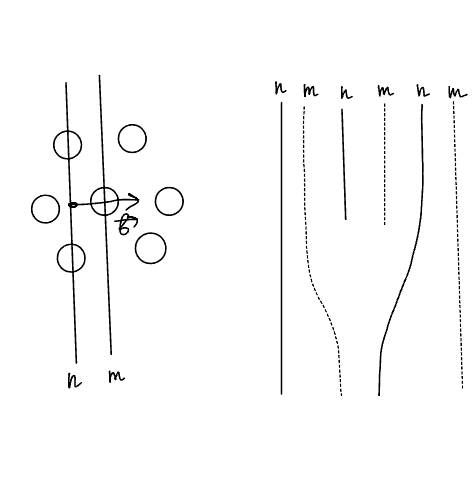
\includegraphics[width=0.55\textwidth]{partial_dislocation.png}\caption{Строение и перемещение краевой дислокации в ГЦК}\label{fig:partial_dislocation}
\end{figure} 
\begin{figure}[h!]
\centering
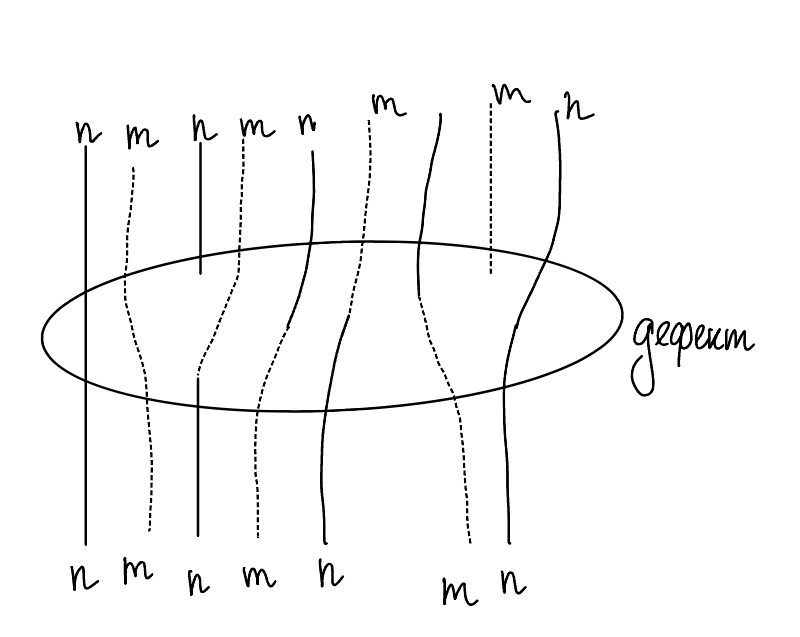
\includegraphics[width=0.55\textwidth]{partial_dislocation_full_view.png}\caption{Дефект упаковки между двумя частичными дислокациями} \label{fig:partial_dislocation_full_view}
\end{figure} 
При движении полной дислокации атомы смещаются между симметрически эквивалентными положениями в структуре. Однако атомы экстраплоскости могут начать перемещаться, "перекатываясь" между ложбинками в укладке слоя. В результате нарушается порядок следования слоёв, образуется дефект упаковки, ограниченный двумя частичными дислокациями (рис. \ref{fig:partial_dislocation_full_view}) с нетрансляционными векторами Бюргерса:
\begin{equation}
  \vec{b}=\vec{b_1}+\vec{b_2}, \text{ }\vec{b_1}\widehat{  }\text{ }\vec{b_2} = 60^\circ
\label{eq:partial_dislocation} 
\end{equation}
Образование дефекта упаковки (т.н. растянутой дислокации) энергетически выгодно, суммарная энергия двух частичных дислокаций меньше, чем энергия одной краевой. Частичные дислокации отталкиваются, однако с увеличением размеров дефекта упаковки растёт его упругая энергия, в результате чего можно говорить о некотором "равновесном" размере дефекта. Упругую энергию дефекта упаковки можно оценить по формуле \ref{eq:Energy_mispacking}.
\begin{equation}
  \gamma = \sigma_1b_2= \frac{G(\vec{b_1},\vec{v_2})}{2\pi l (1-\nu)}
\label{eq:Energy_mispacking} 
\end{equation}
Здесь $\sigma_1$ - поле напряжений, создаваемое первой частичной дислокацией, $l$ - размер дефекта, $\nu$ - коэффициент Пуассона.
\par
\underline{Двойниковый дефект} - это зеркальное расположение атомных плоскостей относительно некоторой плоскости (т.н. двойниковой границы). Может возникать как в результате деформации хрупкого тела, так и непосредственно в ходе роста кристалла. Двойниковые границы называют специальными границами, искажения на таких границах минимальны, равно как и энергия таких границ.
\par ABCBA
\section{Взаимодействие различных дефектов. Модели строения границ зерен.
Сегрегация примесей в поликристаллическом материале.}
Точечные и протяжённые дефекты взаимодействуют друг с другом. Движущая сила этого взаимодействия - минимизация упругой энергии деформации кристаллической решётки. точечные дефекты притягиваются друг к другу. Соприкосновение вакансий выгодно, поскольку снижает число разорванных в веществе связей. Дефекты по Френкелю притягиваются, так как сближение двух пар "междоузельный атом + вакансия" позволяет уменьшить деформацию, создаваемую каждым дефектом в отдельности. Точечные дефекты (в т.ч. атомы примеси) имеют тенденцию скапливаться вблизи протяжённых дефектов в сильнодеформированных областях с образованием атмосферы Коттрелла вокруг дислокаций и атмосферы Судзуки вокруг дефектов упаковки. точечные дефекты могут осаждаться на экстраплоскость, вызывая её переползание перпендикулярно плоскости скольжения дислокации.
\par
Дислокации взаимодействуют друг с другом, знак этого взаимодействия определяется положением дислокаций друг относительно друга. Если поля напряжений и деформаций двух дислокаций гасят друг друга, то такое взаимодействие энергетически выгодно, дислокации притягиваются. В противном случае дислокации отталкиваются. В одной плоскости скольжения дислокации одного знака отталкиваются, разных знаков - притягиваются. Возможны устойчивые конфигурации дислокаций - например, плоское скопление или стенка дислокаций (рис. \ref{fig:dislocation_configurations}).
\begin{figure}[h!]
\centering
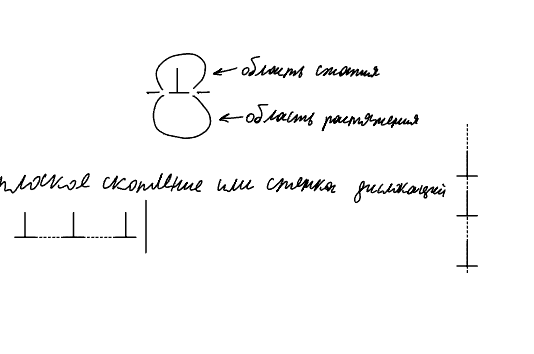
\includegraphics[width=0.55\textwidth]{dislocation_configurations.png}\caption{Примеры устойчивых конфигураций + напряжения вокруг краевой дислокации} \label{fig:dislocation_configurations}
\end{figure} 
\par
Стенка дислокаций фомрирует так называемую малоугловую границу между зёрнами кристалла. Это т.н. граница наклона, когда два зерна развёрнуты друг относительно друга на угол разупорядочения $\theta$ (рис. \ref{fig:misfit_angle}).

\begin{figure}[h!]
\centering
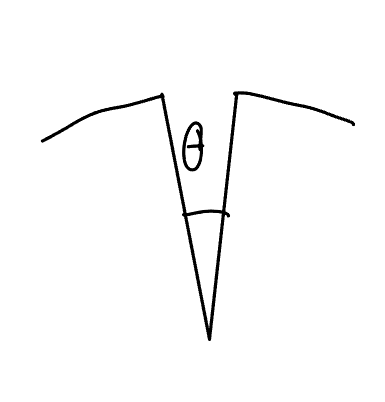
\includegraphics[width=0.3\textwidth]{misfit_angle.png}\caption{Угол разупорядочения} \label{fig:misfit_angle}
\end{figure} 
Существуют также малоугловые границы кручения, образованные серткой винтовых дислокаций. 
\par
При малых углах разориентировки для границ наклона справедлива формула Билби-Франка:
\begin{equation}
 h \approx \frac{b}{\theta}
\label{eq:Bilbi-Frank} 
\end{equation}
Здесь h -расстояние между соседними дислокациями в стенке. При малых $\theta < 15^\circ$ h велико, и ядра дислокаций не перекрываются. Удельная поверхностная энергия такой границы может быть описана формулой 
\begin{equation}
\gamma = \frac{Gb\theta}{4\pi (1-\nu)} \left(\ln \frac{b}{r_0} - \ln \theta \right)
\label{eq:boundary_energetics} 
\end{equation}
Для высокоугловых границ эта модель неприменима, энергия границы зависит от угла, как показано на рис. \ref{fig:boundary_energetics}.
\begin{figure}[h!]
\centering
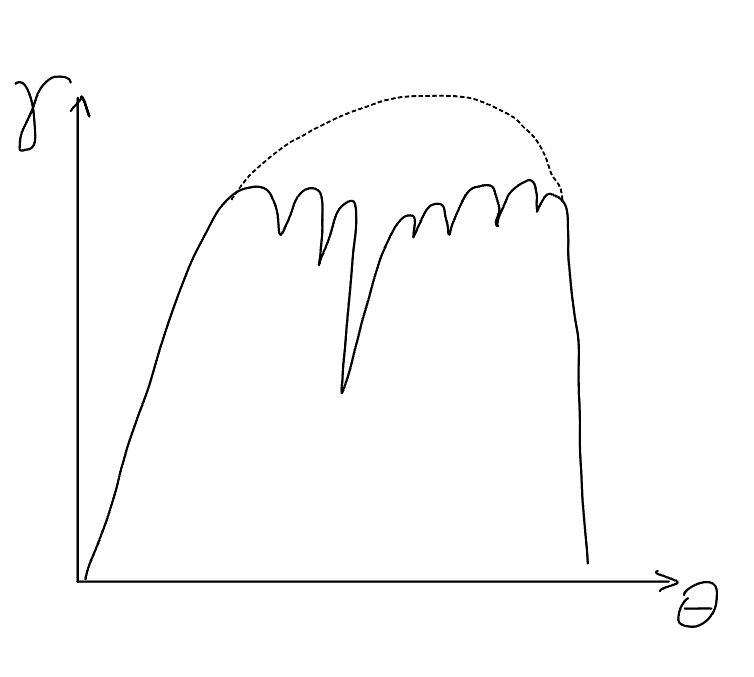
\includegraphics[width=0.3\textwidth]{boundary_energetics.png}\caption{Энергия границы} \label{fig:boundary_energetics}
\end{figure} 
Резкие минимумы энергии отвечают специальным, двойниковым высокоугловым границам. На таких границах наблюдается \underline{решётка совпадающих узлов} с некоторым периодом n. Специальные границы обозначают символом $\Sigma n$, где n -период РСУ. Такое взаиморасположение зёрен требует значительно меньших деформаций, энергетически это выгодно. Между минимумами энергии расположены точки, соответствующие несовершенным высокоугловым границам, для них нет РСУ, просто часть узлов решётки должны совпасть. 
\par
Для описания высокоугловых границ часто используют понятие зернограничных дислокаций, обеспечивающих скольжение зёрен друг относительно друга. Строится решётка зернограничных сдвигов (часть узлов - пусты, в остальных узлах - все атомы, и входящие в РСУ, и не входящие в РСУ). Зернограничные дислокации вводятся в этой решётке и перемещаются в ней. 
\par Вследствие расхождения кристаллических решёток, на границе зерён есть множество мест, в которых энергетически выгодно расположиться крупным примесным атомам (рис. \ref{fig:boundary_sites}).
\begin{figure}[h!]
\centering
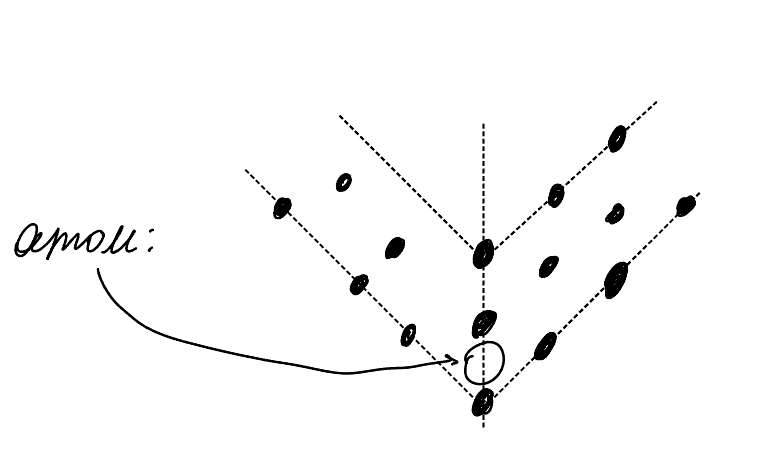
\includegraphics[width=0.3\textwidth]{boundary_sites.png}\caption{К размещению примеси на границе зерён} \label{fig:boundary_sites}
\end{figure} 
\par
Не все примеси склонны сегрегировать к границам зёрен (преимущественно располагаться на них), хотя большинство примесей сегрегирует к границе, такие примеси называют горофильными. Сегрегация примеси обычно описывается уравнением адсорбции Гиббса ($c_i$ - объёмная концентрация вблизи границы):
\begin{equation}
 \Gamma_i = - \frac{c_i}{RT} \left(\frac{\partial \gamma}{\partial c_i} \right)_S
\label{eq:Gibbs_adsorbtion} 
\end{equation}
Чем хуже растворима примесь в веществе, тем сильнее она сегрегирует к границам зёрен. В рамках чисто упругой модели концентрация примеси вблизи границы рассчитывается по формуле 
\begin{equation}
 c_i=c_0e^{-\frac{E}{kT}} \text{, где } E\sim \varepsilon^2
\label{eq:elastic_model_concentrarion} 
\end{equation}
В более сложной модели среднего поля учитывается взаимодействие атомов примеси друг с другом. В этом случае используется изотерма Гугенхейма-Фаулера:
\begin{equation}
 \frac{x}{1-x} = \frac{c_0}{1-c_0}\exp (-\frac{\Delta f +2z\theta x}{kT})
\label{eq:elastic_model_concentrarion}  
\end{equation}
Здесь x - доля занятых позиций на границе, z - КЧ на границе, $\theta = \frac{1}{2} (E^{BB} + E^{AA} - 2E^{AB})$, $\Delta f$ - энергия обмена атомом А на границе с атомом В в объёме. \par
В случае сильного взаимодействия атомов примеси может наблюдаться образование разных поверхностных фаз, напр. - кластеров.
\section{Механизмы зарождения и размножения дислокаций. Механизмы
пластической деформации и разрушения материалов} 
1) Дислокации могут возникать вследствие пластической деформации кристалла. для того, чтобы породить дислокацию, необходимо преодолеть энергетический барьер Пайерлса. Для этого нужно приложить напряжение $\tau>\frac{Gb}{2\pi r_c}$, где $r_c$ - некоторый критический размер ядра дислокации, по достижении которого дислокация образуется.
\par 2) Дислокации могут порождаться вследствие структурного несоответствия двух контактирующих фаз (плёнка+подложка). Это так называемые дислокации несоответствия. Они возникают при превышении толщиной плёнки некоторого критического значения $h_c\approx \frac{b}{9.9 f}$, где $f=\frac{\Delta a}{a}$ - параметр несоответствия.
\par
3) Дислокации возникают при кристаллизации поликристалла с произвольной ориентацией центров кристаллизации вследствие структурного несоответствия на границах зёрен.
\par 4) дислокации могут размножаться, например -  по механизму источника Франка-Рида (рис. \ref{fig:Frank-Reed}). В качестве такого источника выступает закреплённая в двух точках дислокация. Она выгибается под действием внешнего напряжения, пока не примет форму полуокружности при напряжении $\tau \approx \frac{Gb}{L}$, где L - расстояние между точками закрепления.
\begin{figure}[h!]
\centering
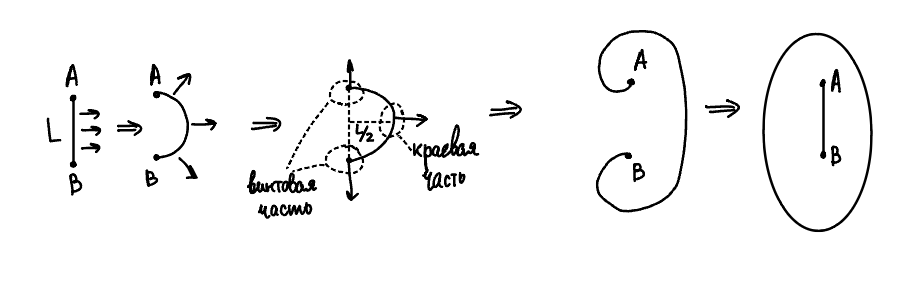
\includegraphics[width=0.9\textwidth]{Frank-Reed.png}\caption{Источник Франка-Рида} \label{fig:Frank-Reed}
\end{figure} 
После этого дислокация самопроизвольно расширяется, пока два участка петли не столкнутся и не с аннигилируют. В результате образуется дислокация между точками АВ и дислокационная петля вокруг источника. Эта петля распространяется по кристаллу, пока не выйдет на его поверхность.
\par
5) Также дислокации могут расщепляться с образованием полных или частичных дислокаций, либо возникать в результате столкновения частичных или полных дислокаций.
\par
Основной механиз пластической деформации - это скольжение дислокаций по плоскостям скольжения. В этом случае на поверхности деформируемого материала наблюдается серия полос (рис. \ref{fig:deformation_patterns}). Хрупкие материалы деформируются за счёт двойникования.
\begin{figure}[h!]
\centering
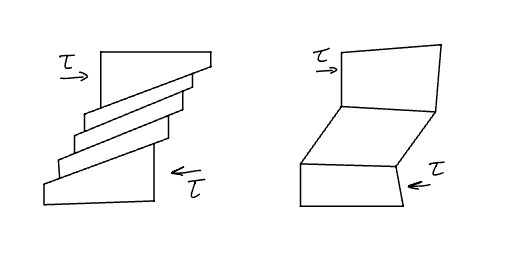
\includegraphics[width=0.5\textwidth]{deformation_patterns.png}\caption{Пластический (слева) и хрупкий (справа) деформацированный материал} \label{fig:deformation_patterns}
\end{figure} 
В случае пластической деформации по механизму скольжения дислокаций, могут активироваться разные системы скольжения. Число возможных систем скольжения определяется кристаллической структурой материала (12 в ГЦК, 3 или 6 в ГПУ). Чем больше возможных систем, тем пластичнее материал. Для каждой плоскости скольжения есть свой  предел текучести:
\begin{equation}
\tau_R = \sigma \cos \varphi \cos \lambda
\label{eq:Schmidt-Boas}  
\end{equation}
Это закон Шмида-Боаса (проекция внешнего напряжения на плоскость скольжения).
\begin{figure}[h!]
\centering
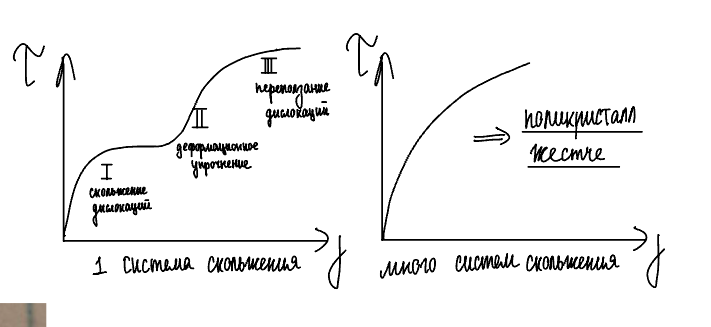
\includegraphics[width=0.7\textwidth]{tension_curve.png}\caption{Кривые нагружения для одной системы скольжения и многих систем скольжения (поликристалл)} \label{fig:tension_curve}
\end{figure} 
Деформационное упрочнение соответствует образованию плоских скоплений дислокаций вблизи границ зёрен.\par
При высоких температурах может наблюдаться  т.н. \underline{высокотемпературная ползучесть} (creep), когда при постоянной нагрузке происходит увеличение $\varepsilon$, поскольку диффузия облегчена (рис. \ref{fig:creep}).
\begin{figure}[h!]
\centering
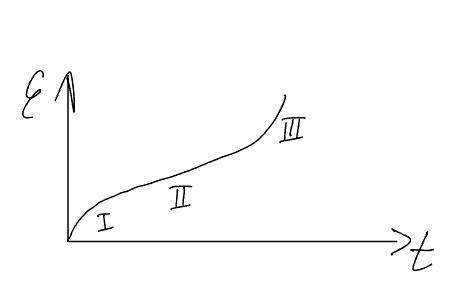
\includegraphics[width=0.3\textwidth]{creep.png}\caption{Зависимость деформации от времени} \label{fig:creep}
\end{figure} 
На рисунке \ref{fig:creep} область I соответствует неустановившейся ползучести (скольжение и генерации дислокации), область II - установившаяся ползучесть (генерация), III - переползание дислокаций, материал разрушается.
\par
В нанокристаллических материалах может наблюдаться сверхпластичность за счёт смещения зёрен друг относителньо друга. 
\par При существенном увеличении $\sigma$ в пластических материалах может наблюдаться диффузионная ползучесть Коббла (по границам зёрен), а при $T\uparrow \uparrow$ - ползучесть Набарро-Херринга, когда деформация происходит засчёт массопереноса в зерне. 
\par
\underline{Разрушение} материалов обычно протекает с образованием трещины. В пластичных материалах в области шейки копятся вакансии, образуются поры, сливаются в трещину, и происходит разрушение. Хрупкие тела разрушаются вокруг опасного дефекта (трещины), без образования шейки. Трещина - это концентратор напряжений, стремится раскрыться, чтобы снизить свою упругую энергию. Однако при раскрытии трещины повышается её поверхностная энергия, поэтому при относительно небольших напряжениях трещина достигает равновесного размера и далее не растёт.
\begin{equation}
\sigma_{\Gamma} = \sqrt{\frac{2E\gamma}{\pi a}}, \text{ где 2a - размер трещины, $\gamma$ - пов. плотн. энергии, Е - модуль Юнга}
\label{eq:Griffits}  
\end{equation}
Однако если в материале есть трещина длиной 2а, а приложенное напряжение превышает критическое напряжение по Гриффитсу ( ур. \ref{eq:Griffits}), то происходит резкий неконтролируемый рост трещины, материал разрушается. Прежде чем достигнуть критического размера, трещина медленно растёт за счёт эффекта среды - разрыва хим. связей в области трещины под малой нагрузкой. \par 
Зародиться трещина может вследствие столкновения дислокаций. 
\par Если материал подвергается знакопеременным нагрузкам, то возможно утсалостное разрушение. В этом случае сперва происходит рост усталостной трещины, например, по механизму Вуда (рис. \ref{fig:Wood_crack}). Трещина достигает критического размера, после чего происходит разрушение. Торец образца выглядит, как на рисунке \ref{fig:crack_fractography}.
\begin{figure}[h!]
\centering
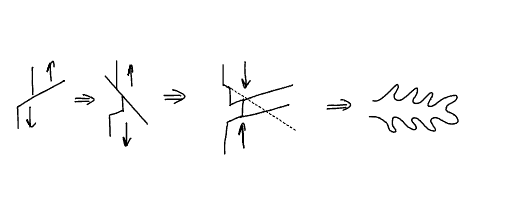
\includegraphics[width=0.7\textwidth]{Wood_crack.png}\caption{Механизм Вуда} \label{fig:Wood_crack}
\end{figure} 
\begin{figure}[h!]
\centering
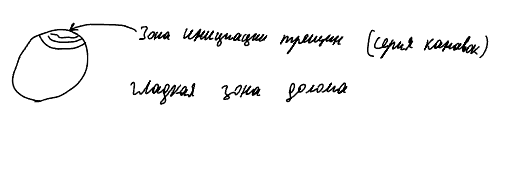
\includegraphics[width=0.7\textwidth]{crack_fractography.png}\caption{Шлиф образца, разрушенного по усталостному механизму}\label{fig:crack_fractography}
\end{figure} 
\section{Механизмы атомно-молекулярных процессов кристаллизации. Зависимости
скорости роста от величины пересыщения в случае нормального роста, спирального
роста (БКФ-механизм), механизма с образованием зародышей (ФКС-механизм).}
Выделяют 3 механизма атомно-молекулярных процессов кристаллизации:\par
1) нормальный рост (подошедшие к поверхности атомы сразу же садятся на шероховатости пов-ти)
\par 2) рост с образованием зародышей (ФКС-механизм, кристалл растёт слой за слоем)
\par3) спиральный рост (БКФ-механизм, атомы садяться во внутренние углы ступенек вышедшей на поверхность винтовой дислокации, кристалл растёт послойно с образованием ростового холма)
\par В случае нормального роста изменение энтропии при кристаллизации невелико, $\Delta_f S < R$. Для этого поверхность кристалла должна быть шероховатой на атомном уровне. Считая, что скорость роста определяется скоростью соударений атомов с поверхностью, можно получить следующее выражение для скорости роста:
\begin{equation}
v = \frac{D_L}{d}(1-e^{-\frac{\Delta G_f}{kT}})
\label{eq:Normal_growth}  
\end{equation}
Это уравнение Вилсона-Френкеля. Здесь $D_L$ - коэффициент диффузии, d - молекулярный/атомный диаметр, $\Delta G_f$ - энергия Гиббса кристаллизации. \par
При малых величинах переохлаждения оно может быть записано в виде 
\begin{equation}
v = \frac{D_L \Delta H_f}{dkT^2}\Delta T \sim \Delta T
\label{eq:Normal_growth_approximation}  
\end{equation}
В случае спирального роста, скорость роста 
\begin{equation}
u \sim f_g \left(1 - \exp \left(-\frac{\Delta H_f \Delta T}{T_m R T} \right) \right)
\label{eq:Spiral_growth}  
\end{equation}
где $f_g \approx \frac{\Delta T}{2 \pi T_m}$ - доля предпочтительных для зародышеобразования мест (сайтов). При малых $\Delta T$ скорость роста $u\sim\Delta T^2$\par
В случае ФКС-механизма (образование зародышей на поверхности, изменение энтропии при кристаллизации весьма велико), атомы могут садиться только в выборочных сайтах. Рост кристалла начинается только при достаточно больших пересыщениях, зависимость скорости роста от $\Delta T$ нелинейная.
\begin{figure}[h!]
\centering
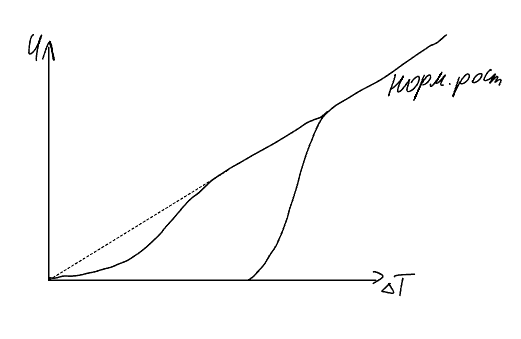
\includegraphics[width=0.4\textwidth]{crystal_growth.png}\label{fig:crystal_growth}\caption{Зависимость скорости роста кристалла от пересыщения для разных механизмов}
\end{figure}
\section{Развитие граней кристалла: теорема Гиббса-Вульфа, габитус кристалла с
точки зрения РВС-теории.}
Скорость роста граней кристалла может быть описана законом Браве: "скорость роста грани обратно пропорциональна плотности её узловой сетки". Огранка кристалла определяется гранями с наименьшими скоростями роста. Быстрорастущие грани как бы <<вытягивают>> медленные (рис. \ref{fig:edge_growth}). Медленнорастущие грани обладают малыми значениями индексов Миллера hkl.
\begin{figure}[h!]
\centering
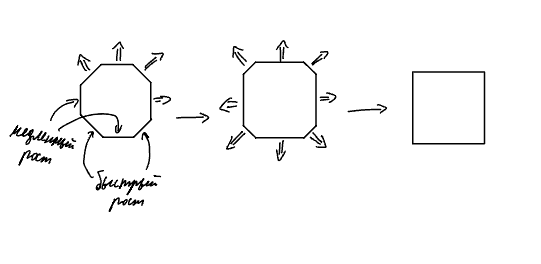
\includegraphics[width=0.5\textwidth]{edge_growth.png}\caption{Влияние скорости роста граней на огранку кристалла}\label{fig:edge_growth}
\end{figure}
Можно рассмотреть термодинамически равновесную огранку кристалла. Для этого решается вариационная задача по минимизации энергии Гиббса образующегося кристалла. В результате можно получить, что
\begin{equation}
\frac{\sigma_i}{r_i} = const \text{ для каждой грани}
\label{eq:Gibbs-Woolf_theorem}  
\end{equation}
Здесь $r_i$ - расстояние от центра кристалла до i-й грани, $\sigma_i$ - удельная поверхностная энергия грани. Это условие носит название \underline{теоремы Гиббса-Вульфа}.\par
В то же время в условиях относительно больших пересыщений включается не термодинамический, а кинетический контроль, существенную роль начинает играть шероховатость растущей грани, определяющая механизм и, следовательно, скорость её роста. Реальная огранка кристалла может отличаться от равновесной. Для описания кинетически контролируемого роста кристаллов построена теория периодической цепи связей (PBC-Theory). В структуре растущего кристалла можно выделить цепочки наиболее интенсивных химических связей, так называемые PBC-цепочки. Чем больше PBC-цепочек в грани, тем более гладкой является грань. Вводится классификация граней:
\par
1) 2 и более PBC-цепочки $\Rightarrow$ F-грани, гладкие, медленнорастущие (ФКС-механизм)
\par
2) 1 PBC-цепочка $\Rightarrow$ S-грани, менее гладкие, реже встречаются в огранке, ибо растут быстрее
\par
3) ни одной PBC-цепочки $\Rightarrow$ K-грани, высокошероховатые, быстро растут по нормальному механизму, в огранке не встречаются.
\begin{figure}[h!]
\centering
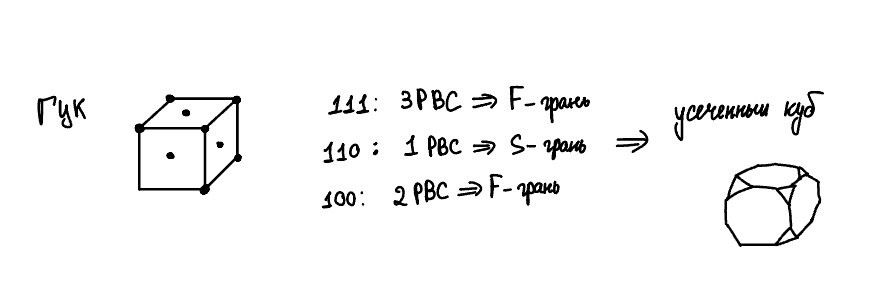
\includegraphics[width=0.7\textwidth]{example_PBC_theory.png}\caption{Пример применения PBC-теории для оценки огранки кристалла} \label{fig:example_PBC_theory}
\end{figure}
\section{Термодинамика выделения фазы, принцип Данкова-Конобеевского.
Гетерогенное зародышеобразование. Переохлаждение и кривизна ростового фронта}
Выделение новой фазы - это фазовый переход I рода, сопровождается скачком первых производных термодинамических потенциалов по интенсивным параметрам:
\begin{equation}
\left(\frac{\partial G}{\partial T}\right)_p = -S; \quad \left(\frac{\partial G}{\partial p}\right)_T = V 
\label{eq:first_derivatives_G_S}  
\end{equation}
Движущая сила процесса - минимизация энергии Гиббса системы. При этом может наблюдаться образование метастабильных фаз, если кинетический фактор (энергетический барьер, связанный с перестройкой структуры) играет значительную роль. Это так называемое правило ступеней Оствальда. 
\par
Изменение энергии Гиббса складывается  из объёмной, поверхностной и упругой составляющих:
\begin{equation}
\Delta G = \underset{<0}\Delta G_{\text{объёмн.}} + \underset{>0}\Delta G_{\text{ поверхн.}} + \underset{>0}\Delta G _{\text{упр.}}
\label{eq:DeltaG_phase_transitions}  
\end{equation}
Поскольку образование новой фазы неизбежно связано с возникновением новых границ раздела, $\Delta G_{\text{поверхн.}}>0$. Для минимизации вклада поверхностной энергии зерно новой фазы стремится к такой ориентации по отношению к исходной фазе, чтобы  рассогласование кристаллических решёток было минимальным. В этом и заключается так называемый \underline{принцип Данкова-Конобеевского}. При образовании новой фазы из расплава $\Delta G_{\text{упр.}}=0$, поэтому конкурируют только объёмная и поверхностная энергии. В случае \underline{гетерогенного зародышеобразования} в системе изначально присутствуют поверхности, обладающие избытком свободной энергии. В результате $\Delta G_{\text{поверхн.}}$ меньше, чем в случае гомогенного зародышеобразования, и рост кристаллов происходит при меньших значениях переохлаждения $\Delta T$.
\par
При гомогенном зародышеобразовании $\Delta G_{\text{объёмн.}}$ не сразу может преодолеть вклад от $\Delta G_{\text{поверхн.}}$, в результате зародыш обладает избытком энергии Гиббса, и кристаллизация идёт через потенциальный барьер (см. рис. \ref{fig:crystallization_barrier}):
\begin{equation}
\Delta G_c \sim \frac{1}{\Delta T}, r_c \sim \frac{1}{\Delta T}
\label{eq:crystallization_energy_barrier}  
\end{equation}
\begin{figure}[h!]
\centering
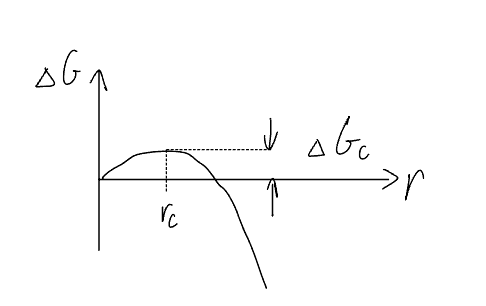
\includegraphics[width=0.3\textwidth]{crystallization_barrier.png}\caption{Потенциальный барьер кристаллизации} \label{fig:crystallization_barrier}
\end{figure}
$r>r_c \Rightarrow$ кристалл растёт, $r<r_c \Rightarrow$ зародыш растворяется.
\par При гетерогенном зародышеобразовании $r_c$ не меняется, а величина барьера уменьшается и становится равной
\begin{equation}
\Delta G_{het} = \Delta G_c (2-3\cos \theta + \cos^3\theta)
\label{eq:heterocrystallization_energy_barrier}  
\end{equation}
Здесь $\theta$ - это угол смачивания между зародышем и подложкой. Необходимо добиться такой величины $\Delta T$, чтобы случайно образующиеся зародыши могли вырасти.
\par
В то же время, высокие значения $\Delta T$ способны привести к нестабильности ростового фронта. Для роста искривлённой поверхности требуется меньшее пересыщение, чем для роста прямой поверхности. Малые выступы, образующиеся на ростовом фронте, превышают критический размер и начинают расти, поверхность роста искривляется. Чем сильнее изгибается фронт, тем меньшие переохлаждения требуются для его дальнейшего роста. Соответственно, тем больше получается актуальное переохлаждение вблизи границы. В результате происходит рост дендритов (рис. \ref{fig:dendrites_growth}) с последующим отрывом их от ростовой поверхности кристалла. Процесс нежелательный.
\begin{figure}[h!]
\centering
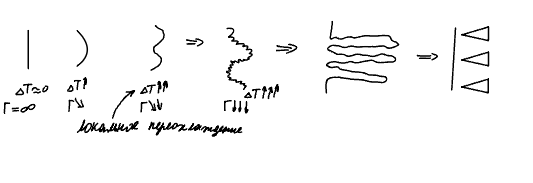
\includegraphics[width=0.85\textwidth]{dendrites_growth.png}\caption{Рост дендритов} \label{fig:dendrites_growth}
\end{figure}
\section{Распределение примеси по длине растущего из расплава кристалла.
Техническое оформление основных методов роста кристаллов из расплава.}
Вследствие несовпадения составов расплава и растущего кристалла (линии ликвидуса и солидуса на фазовой диаграмме не совпадают), состав расплава по мере роста кристалла непрерывно меняется (рис. \ref{fig:liquation_crystal_growth}). 
\begin{figure}[h!]
\centering
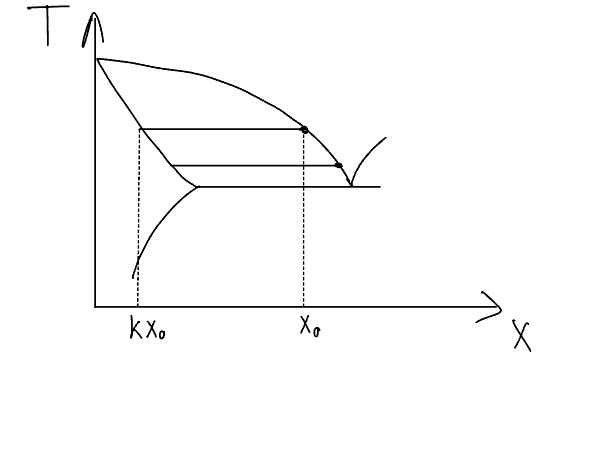
\includegraphics[width=0.3\textwidth]{liquation_crystal_growth.png}\caption{Причина непостоянства концентрации примеси в кристалле}\label{fig:liquation_crystal_growth}
\end{figure}
\begin{figure}[h!]
\centering
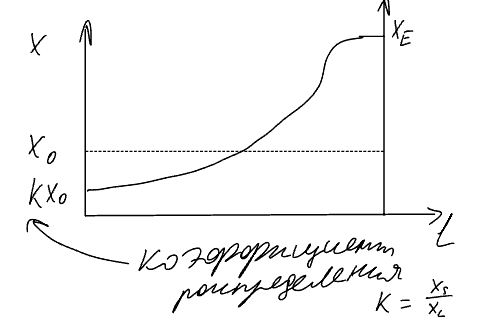
\includegraphics[width=0.5\textwidth]{c(x)_crystal.png}\caption{Зависимость концентрации примеси в кристалле от координаты}\label{fig:c(x)_crystal}
\end{figure}
В результате непрерывно меняется и состав растущего кристалла, так что в конечном итоге распределение примеси по кристаллу имеет вид, показанный на рис. \ref{fig:c(x)_crystal}. 
\par Коэффициент распределения $k=\frac{x_s}{x_L}\approx const$ для линейных ликвидуса и солидуса. Вид кривой x(l) получается при интегрировании выражения 
\begin{equation}
(x_L-x_S)df_S=(1-f_S)dx_L \text{   - принцип сохранения примеси}
\label{eq:impurity_conservation}  
\end{equation}
Здесь $f_S$ - объёмная доля кристалла (по сути - координата границы раздела). В результате получаем уравнение темпа кристаллизации:
\begin{equation}
x_S = kx_0 (1-f_S)^{k-1} = kx_0 (1-l)^{k-1} 
\label{eq:crystallization_rate}  
\end{equation}
Для того, чтобы избежать столь существенных неоднородностей состава (рис. \ref{fig:c(x)_crystal}), можно осуществлять подпитку расплава примесью, загружая в расплав шихту смеси компонентов состава $x_0$. В этом случае с учётом диффузии в расплаве получаем следующее распределение примеси по расплаву (рис. \ref{fig:c(x)_fusion}):
\begin{figure}[h!]
\centering
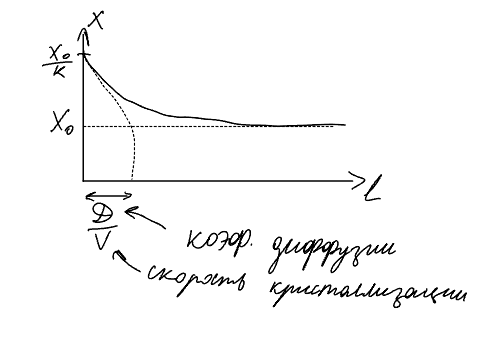
\includegraphics[width=0.5\textwidth]{c(x)_fusion.png}\caption{Зависимость концентрации примеси в расплаве от координаты}\label{fig:c(x)_fusion}
\end{figure}
\parИ, как следствие, такое распределение примеси по кристаллу (рис \ref{fig:c(x)_crystal_normal}):
\begin{figure}[h!]
\centering
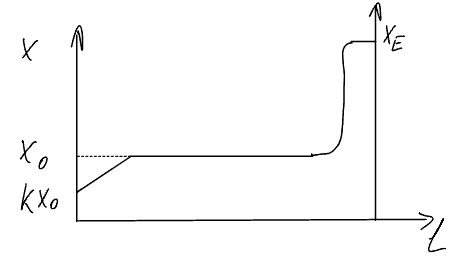
\includegraphics[width=0.5\textwidth]{c(x)_crystal_normal.png}\caption{Зависимость концентрации примеси в кристалле от координаты с учётом диффузии в расплаве}\label{fig:c(x)_crystal_normal}
\end{figure}
\par Начальная и конечная области отрезаются, остаётся однородный кристалл.
\par \underline{Основные методы роста кристаллов из расплава}:
\par 1) Бриджмен-Стокбаргер (движение расплава в температурном градиенте, рис. \ref{fig:Bridgeman_Stockbarger})
\par 2) Чохральский (вытягивание вращающейся затравки из расплава, рис. \ref{fig:Bridgeman_Stockbarger})
\par 3) Зонная плавка (рис. \ref{fig:zone_fusion})
\par 4) Вернейль (в пламени, для тугоплавких материалов, рис. \ref{fig:zone_fusion})
\par 5) Массовая и спонтанная кристаллизация 
\begin{figure}[h!]
\centering
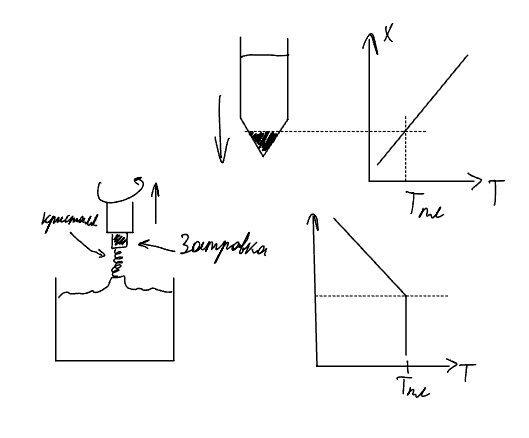
\includegraphics[width=0.4\textwidth]{Bridgeman-Stockbarger.png}\caption{Метод Бриджмена (сверху) и Чохральского (снизу)}\label{fig:Bridgeman_Stockbarger}
\end{figure}
\begin{figure}[h!]
\centering
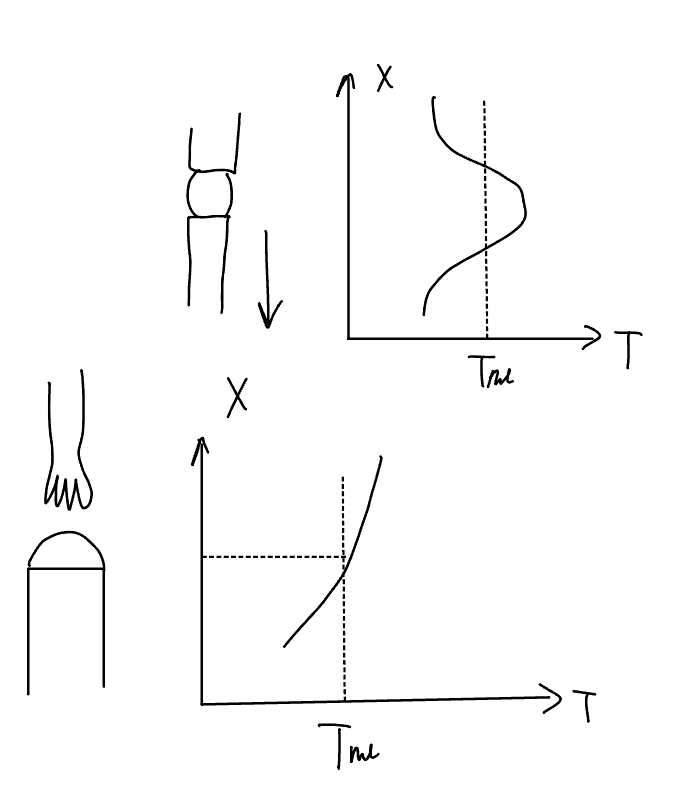
\includegraphics[width=0.4\textwidth]{zone_fusion.png}\caption{Метод зонной плавки (сверху) и Вернейля (снизу)}\label{fig:zone_fusion}
\end{figure}
\section{Направленная кристаллизация. Условие стабильности интерфейса при
направленной кристаллизации. Теория эвтектического роста.}
Направленная кристаллизация осуществляется следующим образом. на границу раздела кристалл/расплав подаётся температурный градиент, через который с некоторой скоростью v протягивается образец. v соответствует скорости кристаллизации. Важно, чтобы переохлаждение вблизи границы раздела было невелико, в противном случае можно получить нестабильность ростового фронта ($R\sim \frac{1}{\Delta T}$, R - радиус кривизны, $\Delta T$ - локальное переохлаждение). Для этого тепло должно отводиться через кристалл.
\par В случае направленной кристаллизации распределение примеси по расплаву имеет следующий вид (рис. \ref{fig:x(l)_crystal_melt}):
\begin{figure}[h!]
\centering
\centering
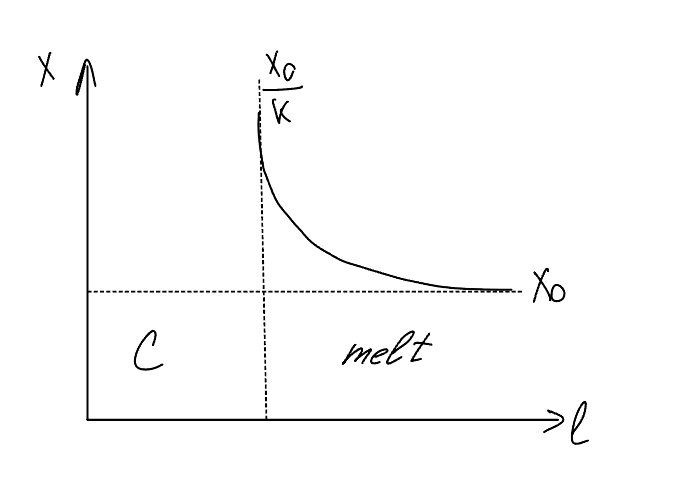
\includegraphics[width=0.2\textwidth]{x(l)_crystal_melt.png}\caption{Распределение примеси в кристалле и в расплаве вблизи границы раздела} \label{fig:x(l)_crystal_melt}
\end{figure}
\par  Каждой концентрации примеси можно сопоставить равновесную температуру, отвечающую данному составу на фазовой диаграмме. Если наложенный температурный градиент слишком мал (рис. \ref{fig:concentrational_undercooling}), то вблизи поверхности раздела раствор пересыщен, наблюдается так называемое концентрационное переохлаждение, которое способно привести к нестабильности ростового фронта точно также, как и обычное термическое. 
\begin{figure}[h!]
\centering
\centering
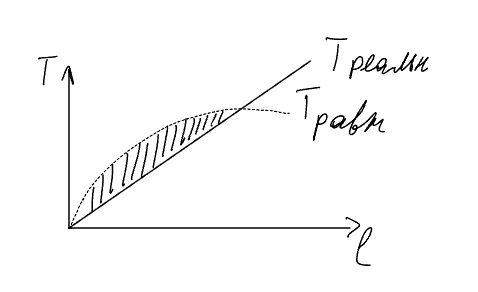
\includegraphics[width=0.3\textwidth]{concentrational_undercooling.png}\caption{К понятию концентрационного переохлаждения} \label{fig:concentrational_undercooling}
\end{figure}
\par Для стабильности ростового фронта важно, чтобы при росте кристалла скорость кристаллизации и температурный градиент были сбалансированы во избежание концентрационного переохлаждения. Условие стабильности ростового фронта записывается следующим образом:
\begin{equation}
\frac{\nabla T}{v}\geq \frac{-m_Lx_0(1-k)}{D_L} 
\label{eq:growth_stability}  
\end{equation}
Здесь $D_L$ - коэффициент диффузии в расплаве, $k=\frac{x_S}{x_L}$ - коэффициент распределения, $m_L<0$ - наклон ликвидуса (в линейной модели ликвидуса и солидуса).
\par
\underline{Кристаллизация эвтектик} описывается теорией Джексона-Ханта. В рамках этой теории распределение примеси по кристаллу описывается уравнением
\begin{equation}
\frac{\partial^2C}{\partial^2x}+\frac{\partial^2C}{\partial^2y}+\frac{v}{D}\frac{\partial C}{\partial z} = 0
\label{eq:Jackson-Hant_concentration}  
\end{equation}
Это означает, что распределение примеси по кристаллу в направлении z периодично. При кристаллизации эвтектики расплав пересыщен относительно обеих фаз сразу (рис. \ref{fig:eutectic_crystal}), так что обе фазы кристаллизуются одновременно с образованием стопки пластин-ламелей с дифференцировкой $\lambda$. 
\begin{figure}[h!]
\centering
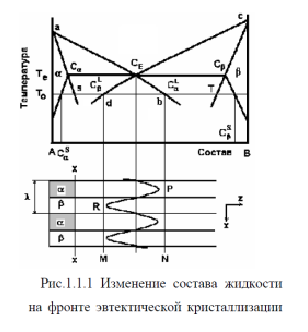
\includegraphics[width=0.5\textwidth]{eutectic_crystal.png}\caption{Переохлаждение и кристаллизация эвтектики}\label{fig:eutectic_crystal}
\end{figure}
\par Для того, чтобы движущая сила кристаллизации была отлична от нуля, требуется некоторое переохлаждение на границе, которое складывается из концентрационного переохлаждения (при образовании пластины одной фазы раствор обогащается вторым компонентом) и переохлаждения, связанного с кривизной ростового фронта:
\begin{equation}
\Delta T = Av\lambda + \frac{B}{\lambda}
\label{eq:eutectic_undercooling}  
\end{equation}
Первое слагаемое отвечает концентрационному переохлаждению, второе - переохлаждению за счёт кривизны ростового фронта.
\par Условие планарности ростового фронта эвтектического кристалла ($\Delta T \rightarrow min$): 
\begin{equation}
\lambda^2v=const
\label{eq:eutectic_planar_face1}  
\end{equation}
\begin{equation}
\frac{(\Delta T)^2}{v}=const
\label{eq:eutectic_planar_face2}  
\end{equation}
\begin{equation}
\Delta T \lambda = const
\label{eq:eutectic_planar_face3}  
\end{equation}
\section{Фазовые равновесия. Основные понятия: система, компонент, фаза,
степень свободы. Условия равновесия фаз. Правило фаз Гиббса. Фазовые
диаграммы Т-х двухкомпонентных систем.}
Фазовые равновесия - это равновесия между фазами в термодинамической системе. \underline{Термодинамическая система} - это материальный объект, выделенный из окружающей среды с помощью реально существующей или воображаемой границы. \underline{Компонентами} называют минимальный набор составляющих (реальные вещества/частицы, образующие систему), достаточный для описания состава системы.
\par
\underline{Пр.} $\rm CO, CO_2, O_2 \Rightarrow$ 3 составляющих, 2 компонента (ибо $\rm CO + \frac{1}{2}O_2=CO_2$)
\par
\underline{Фаза} - гомогенная часть гетерогенной системы, отделённая от других частей границей раздела, при переходе через которую свойства системы меняются скачком. \par
\underline{Степень свободы} - это параметр, который можно независимо менять, оставаясь при этом в пределах одной и той же фазы. Число степеней свободы (ЧСС) - количество таких независимых параметров.
\par С течением времени система может прийти в состояние термодинамического равновесия, когда внутри системы  не будет наблюдаться потоков вещества и энергии, и характеристики системы станут постоянными. В этом случае для фаз, составляющих систему, можно записать частные условия равновесия:
\begin{equation}
T^\alpha=T^\beta; p^\alpha = p^\beta; \mu_i^\alpha = \mu_i^\beta
\label{eq:partial_equilibrium_conditions}  
\end{equation}
То есть, во всех фазах должно соблюдаться равенство температур (термическое равновесие), давлений (механическое равновесие) и химических потенциалов каждого из компонентов (химическое равновесие). 
\par Правило фаз Гиббса связывает число степеней свободы $f$ с количеством равновесных фаз Ф в К-компонентной системе:
\begin{equation}
f=K-\Phi+N
\label{eq:Gibbs_rule}  
\end{equation}
Здесь N - число внешних управляющих факторов (p, T, $\vec{B}$, $\vec{g}$...). Обычно N=2, так как ключевую рлль играют p и Т.
\par ДЛя описания двухкомпонентных систем часто прибегают к использованию Т-х диаграмм, представляющих собой сечения р-Т-х диаграмм при постоянном давлении (обычно 1 атм.). В этом случае $f=K-\Phi+1$. Общий вид Т-х диаграммы показан на рисунке \ref{fig:T-x_diagram}.
\begin{figure}[h!]
\centering
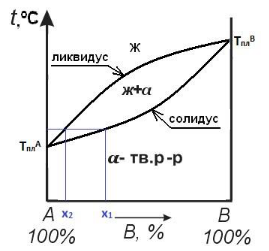
\includegraphics[width=0.3\textwidth]{T-x_diagram.png}\caption{Фазовая диаграмма двухкомпонентной системы}\label{fig:T-x_diagram}
\end{figure}
Для примера приведена Т-х диаграмма, описывающая систему двух неограниченно растворимых друг в друге компонентов. В областях ж и $\alpha$ $\Phi=1 \Rightarrow f=2$, можно менять Т и состав. В области двухфазного равновесия $f=1$, независимо можно менять только температуру, составы фаз жёстко связаны друг с другом.
\section{Основные виды конгруэнтных и инконгруэнтных равновесий. Правило
рычага. Способы графического изображения фазовых диаграмм
трехкомпонентных систем. Квазибинарные разрезы. Принцип триангуляции.} 
Равновесие называется конгруэнтным, если составы равновесных фаз совпадают. В противном случае равновесие называют инконгруэнтным. Трёхфазные равновесия делят на два больших типа: эвтектические (фаза при охлаждение распадается на две) и перитектический (фаза при нагревании распадается на две). В зависимости от состояния фаз (тв., ж., г.) различают следующие равновесия (рис. \ref{fig:phase_equilibrium_types}):
\begin{figure}[h!]
\centering
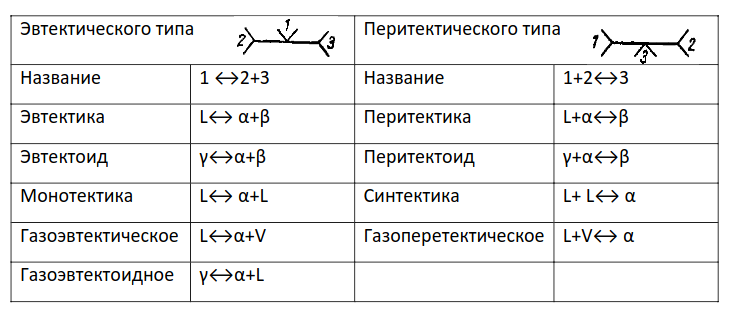
\includegraphics[width=0.8\textwidth]{phase_equilibrium_types.png}\caption{Типы трёхфазных равновесий}\label{fig:phase_equilibrium_types}
\end{figure}
\par Правило рычага позволяет найти соотношение между количеством двух равновесных фаз и их составом (рис. \ref{fig:lever_rule}, n - количество фазы, моль. x - мольная доля одного из компонентов):
\begin{figure}[h!]
\centering
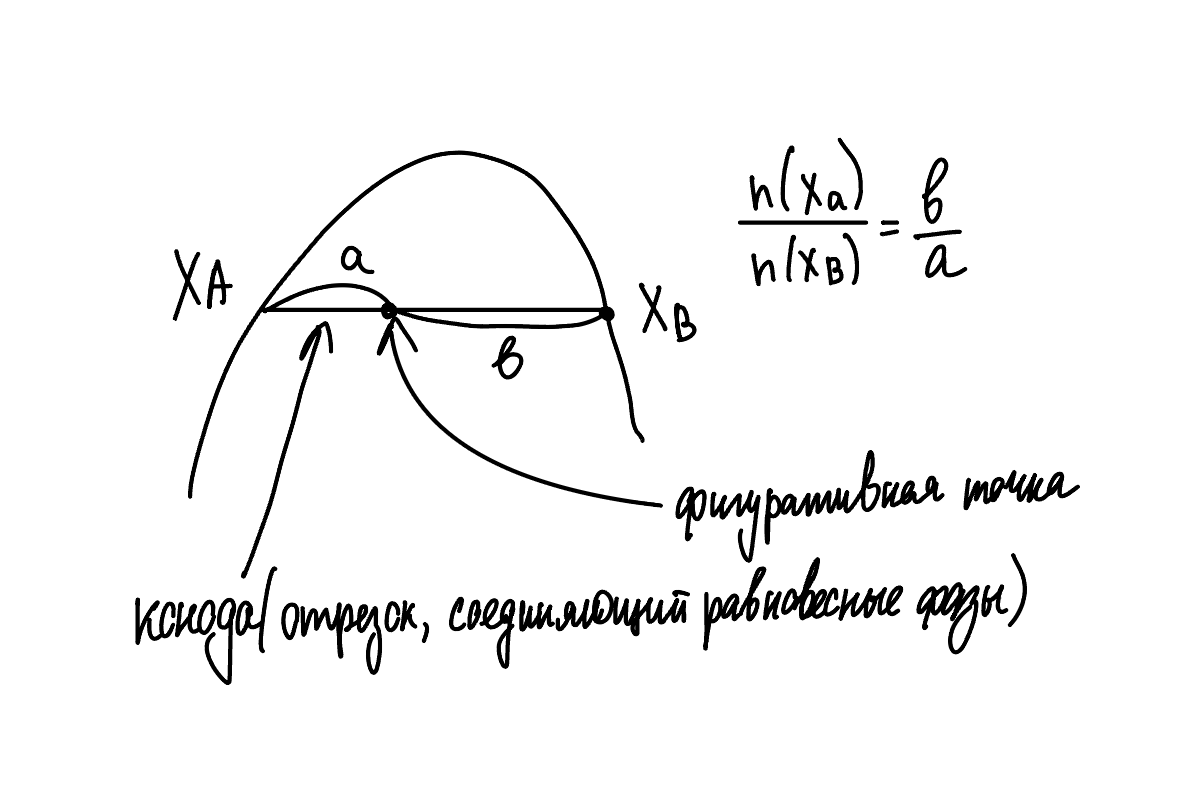
\includegraphics[width=0.6\textwidth]{lever_rule.png}\caption{Правило рычага}\label{fig:lever_rule}
\end{figure}
\par Для изображения фазовых диаграмм трёхкомпонентых систем часто используют треугольник составов Гиббса-Розенбома, который помещают в основание трёхмерной Т-х1-х2-х3 диаграммы при р=const (обычно 1 атм.). Чаще всего пользуются изотермическими сечениями таких диаграмм. Ещё используют развёртки трёхмерных диаграмм, а также их политермические разрезы. 
\par \underline{Квазибинарный разрез} - это политермический разрез, построенный вдоль отрезка, соединяющего на треугольнике составов два конгруэнтно плавящихся соединения, сосуществующих в данной системе (рис. \ref{fig:quasibinary}).
\begin{figure}[h!]
\centering
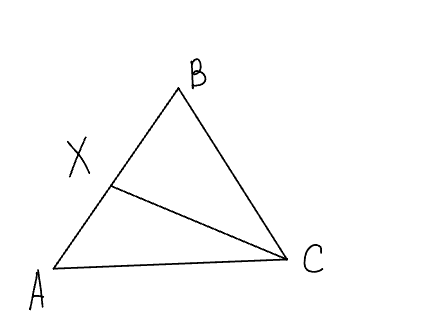
\includegraphics[width=0.3\textwidth]{quasibinary.png}\caption{Квазибинарный разрез}\label{fig:quasibinary}
\end{figure}
\par Можно показать, что смешением С и Х можно получить только точки, принадлежащие отрезке СХ, так что квазибинарное сечение по сути представляет собой двухкомпонентную фазовую диаграмму. При этом важно, чтобы фазы С и Х могли сосуществовать пр данных условиях (т.н. термодинамический критерий выбора квазибинарного разреза). В отдельных случаях при превышении некоторого температурного предела квазибинарный разрез может перестать быть таковым, ибо пройдут процессы химического превращения С и Х с образованием новых фаз.
\par Для изотермических сечений используется принцип триангуляции. Поскольку $p=const, T=const$, то $f=K-\Phi \Rightarrow max\Phi=K=3$. Это означает, что в равновесии может находиться не более трёх фаз. Если в результате некоторого процесса в системе К1-К2-К3 (рис. \ref{fig:triangulation}) получен образец (точка М), содержащий фазы А,В и С, отвечающие некоторым конгруэнтно плавящимся соединениям, присутствующим в данной системе, то треугольник АВС представляет собой область нонвариантного равновесия и не содержит иных фаз, кроме А, В и С. 
\par Такой подход к изучению фазовых диаграмм позволяет разбивать их на простейшие треугольники с тройной эвтектикой, проводить триангуляцию. Этот метод требует больших временных затрат, но позволяет максимально подробно описывать систему.
\begin{figure}[h!]
\centering
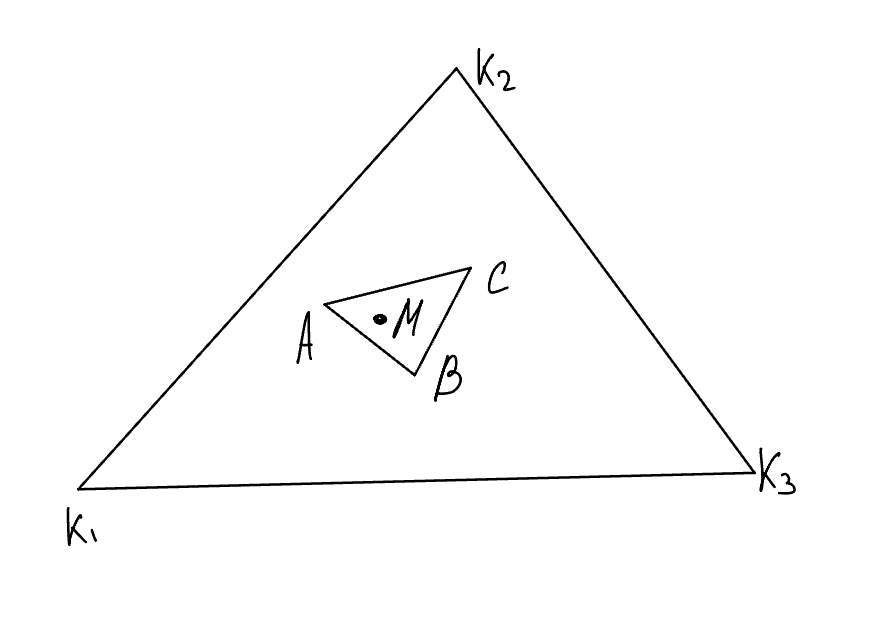
\includegraphics[width=0.4\textwidth]{triangulation.png}\caption{Процесс триангуляции} \label{fig:triangulation}
\end{figure}
\section{Фазовая диаграмма и микроструктура материала. Микроструктура
эвтектических и перитектических композитов. Ликвация и ее влияние на
микроструктуру материала}
По фазовой диаграмме системы можно понять последовательность процессов, происходящих при охлаждении расплава заданного состава $x_0$. Например, если кристаллизация проводится в системе с эвтектикой по пути, показанному на рис. \ref{fig:crystallization_path_eutectic}, то сперва кристаллизуются зёрна фазы $\alpha$, причём состав зерна меняется от ядра к поверхности.
\begin{figure}[h!]
\centering
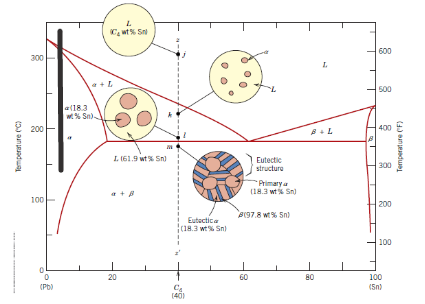
\includegraphics[width=0.6\textwidth]{crystallization_path_eutectic.png}\caption{Кристаллизация сплавов в системе с эвтектикой}\label{fig:crystallization_path_eutectic}
\end{figure}
По достижении температуры эвтектики между зёрнами фазы $\alpha$ кристаллизуется композит эвтектического состава. В результате сплав обладает микроструктурой, показанной на рис. \ref{fig:crystallization_path_eutectic} и характеризуется повышенной прочностью. 
\par
Если кристаллизацию вести по другому пути (рис. \ref{fig:crystallization_path_eutectic}, жирная чёрная линия слева), то будет получен однофазный пластичный материал из зёрен фазы $\alpha$. Если кристаллизуется эвтектический состав, будет получен чисто эвтектический композит \textit{(микроструктура как на рисунке, только без зёрен фазы $\alpha$, просто пластинки в зёрнах)}
\par
Если в системе есть перитектическое равновесие (например - перитектоид, как на рис. \ref{fig:crystallization_path_peritectic}), то по мере охлаждения расплава сперва будут образовываться зёрны фазы $\alpha$, а затем в них произойдёт выделение мелких зёрен фазы $\beta$, в результате чего прочность материала вырастет, а микроструктура будет иметь вид, показанный на рис. \ref{fig:crystallization_path_peritectic}.
\begin{figure}[h!]
\centering
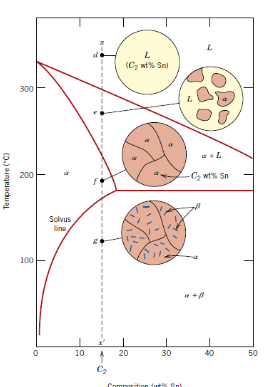
\includegraphics[width=0.4\textwidth]{crystallization_path_peritectic.png}\caption{Кристаллизация сплавов в системе с перитектоидом}\label{fig:crystallization_path_peritectic}
\end{figure}
\par Вследствие несовпадения составов расплава и растущего кристалла (линии солидуса и ликвидуса не совпадают) состав кристалла по мере роста непрерывно меняется (рис. \ref{fig:liquation}).
\begin{figure}[h!]
\centering
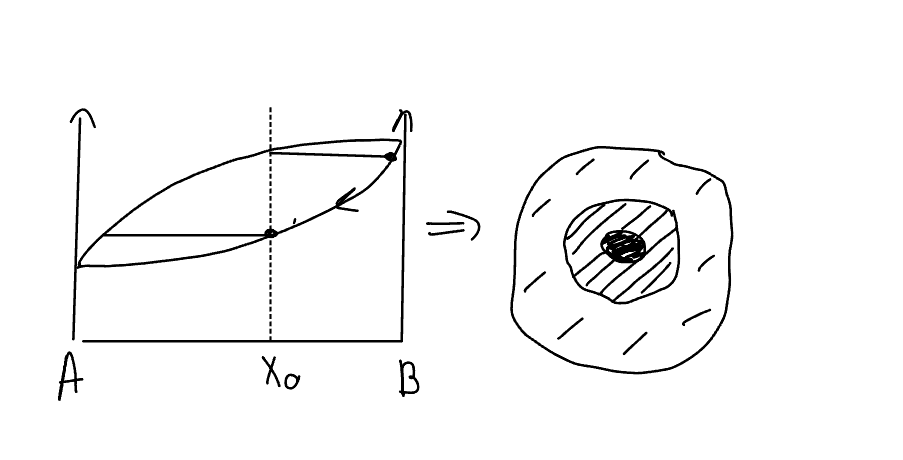
\includegraphics[width=0.8\textwidth]{liquation.png}\caption{Ликвация}\label{fig:liquation}
\end{figure}
В результате ядро зерна обогащено компонентом В, а внешняя область - обеднена, чтобы в среднем состав соответствовал $x_0$. Неоднородность распределения примеси, вызванная различной растворимостью примеси в кристалле и расплаве, наз. ликвацией. Особенно заметно это явление в массивных отливках, где кристаллизация идёт от стенок и дна формы к верхней части. Ликвация приводит к снижению прочности материала, бороться с ней можно путём диффузионного отжига либо замедленного литья.
\section{Закалка без полиморфного превращения. Закалка на мартенсит.
Кристаллогеометрия и термодинамика мартенситного превращения.}
Закалка без полиморфного превращения - это резкое охлаждение образца, при котором замораживаются диффузионные процессы и фиксируется высокотемпературный фазовый и химический состав, а также распределение дефектов. Для достижения этого эффекта металлические сплавы обычно закаляют со скоростями $\sim 1000 ^\circ C/\text{сек}$. для сохранения метастабильной аморфной структуры стекла требуются значительно меньшие скорости закалки. Закалка, проводимая непосредственно из расплава, позволяет избежать ликвации.
\par
В некоторых случаях ($\gamma$-Fe, $\rm ZrO_2$) при закалке происходит бездиффузионное, деформационное превращение с образованием новой фазы того же хим. состава. Кристаллы новой фазы растут со скоростями порядка скорости звука в твёрдом теле. Такое превращение называют мартенситным переходом. Этот процесс наблюдается в определённом интервале температур $T_\text{н}-T_\text{к}$ и полностью протекает только при достижении $T_\text{к}$, что не всегда возможно. 
\par
Мартенситный переход (МП) - деформационный, связан с малыми смещениями атомов кристаллической решётки исходной фазы. Соответственно, мартенситная фаза строго ориентирована по отношению к исходной. Плоскость сопряжения кристаллический решёток фаз при этом не деформируется (МП - т.н. "превращение с инвариантной плоскостью"). В зависимости от того, какой последовательностью девормаций описывается МП, вводятся различные ориентационные соотношения, связывающие некоторые направления и плоскости в исходной и мартенситной фазе. В частности, известны ориентационные соотношения Бейна, Курдюмова-Закса, Нишиямы и т.д.
\par \underline{Пр.} Соотношения Курдюмова-Закса: $(111) \parallel (101)$, то есть плоскости плотнейшей упаковки в ГЦК и ОЦТ параллельны.
\par
Энергия Гиббса МП может быть записана в виде
\begin{equation}
\Delta G_{\text{МП}} = \underset{<0}\Delta G_{\text{объёмн.}} + \underset{>0}\Delta G_{\text{ поверхн.}} + \underset{\gg 0}\Delta G _{\text{упр.}}
\label{eq:Gibbs_martensite}  
\end{equation}
В равновесии $\Delta G_{\text{объёмн.}}+ \Delta G_{\text{поверхн.}}= -\Delta G _{\text{упр.}}$. Управляя внешней нагрузкой, наложенной на материал, можно управлять количеством мартенситной фазы (через изменение $T_\text{н}$).
\section{Мартенситные превращения в металлических и неметаллических
системах, их влияние на механические свойства материалов (изменение
механических характеристик сталей при закалке, трансформационное
упрочнение керамики на основе $\rm ZrO_2$).}
МП - это резкий ($v\sim 1$ км/с) рост кристаллов новой метастабильной фазы внутри зёрен исходной фазы, протекающий при закалке материала ниже некоторой температуры $T_\text{н}$. Мартенситное превращение имеет деформационный характер, связано с малыми смещениями атомов в кристаллической решётки исходной фазы. 
\par Зёрна мартенситной фазы имеют вид протяжённых плоскостей (высокоуглеродистые стали) или плотноупакованных реек (легированные малоуглеродистые стали), разрезающих зерно исходной фазы. В результате происходит существенное повышение прочностных характеристик материала, таких как твёрдость по Бринеллю или временное сопротивление разрыву.
\par
Механизм упрочнения: 1) По Холлу-Петчу 2) дислокационное упрочнение на границах зёрен (МП приводит к значительному увеличению количества дислокаций и двойниковых дефектов в материале). \par С ростом доли углерода в сталях прочность и твёрдость растут, но при выходе за эвтектоидный состав выходят на плато, а прочность может демонстрировать даже падение. Это вызвано образованием зёрен хрупкого цементита $\rm Fe_3C$ (закалка ведётся из двухфазной области, если $x>x_E$).
\par Закалённая сталь - очень напряжённый и потому хрупкий материал. Для дальнейшего использования сталь обычно остаривают, вследствие чего доля мартенсита снижается, равно как и твёрдость с прочностью. зато получается менее хрупкий материал.
\par
МП могут протекать не только в сталях. Примеры: графит$\rightarrow$алмаз, NiTi (ОЦК$\rightarrow$ромбоэдр), BN(гекс.$\rightarrow$куб.), $\beta$-Sn$\rightarrow$$\alpha$-Sn (тетрагон.$\rightarrow$куб. при 13,2 $^\circ C$).
\par В некоторых случаях такие МП вредны (оловянная чума), но могут быть и весьма полезны. Например, МП приводит к деформационному упрочнению $\rm ZrO_2$. В диоксиде циркония возможен МП от тетрагональной фазы к моноклинной. Когда в керамике на основе $\rm ZrO_2$ начинает распространяться трещина, вблизи её края деформации вызывают МП в зёрнах $\rm ZrO_2$. В результате трещина упирается в зерно мартенситной моноклинной фазы, образующееся вследствие МП поле упругих напряжений стремится схлопнуть трещину, и её рост замедляется. Это позволяет использовать $\rm ZrO_2$ в качестве шаров в шаровых мельницах, керамических режущих инструментов и т.д.
\section{Фазовые превращения с норма льной кинетикой. Перлитное
превращение в сталях. ТТТ-диаграмма. Основные разновидности отжига 2 -го
рода}
К фазовым превращениям с нормальной кинетикой (не деформационное, а относительно медленное превращение) относится перлитное превращение в сталях. Это переход аустенита в перлит (эвтектический композит феррита $\alpha$-Fe и цементита $\rm Fe_3C$) при охлаждении. Если распадается аустенит гипо- или гиперэвтектоидного состава, то помимо эвтектоидного композита будут наблюдаться крупные зёрна $\alpha$-Fe или пластинчатые зёрна $\rm Fe_3C$, соответственно. Пластинки цементита играют роль концентраторов напряжений, поэтому для заэвтектоидных сталей характерно снижение прочности (хотя в доэвтектоидных с ростом доли С прочность растёт).
\par Положением эвтектоидной точки можно управлять, добавляя легирующие добавки.
\par Mn, Ni, Co: $T_E\downarrow$ 
\par Cr, Ti, W, Mo, Si: $T_E\uparrow$
\par Ti: $x_E\downarrow \downarrow$
\par Ni, Cr: $x_E\downarrow$
\par
\begin{equation}
\Delta G_{\text{МП}} = \underset{<0}\Delta G_{\text{объёмн.}} + \underset{>0}\Delta G_{\text{ поверхн.}} + \underset{>0}\Delta G _{\text{упр.}}
\label{eq:Gibbs_perlite}  
\end{equation}
Необходимо, чтобы $|\Delta G_{\text{объёмн.}}|$ было достаточно велико. Для этого требуются пониженные температуры ($T \ll T_E$). Но при низких T заторможены процессы диффузии! В результате $\exists$ некая оптимальная Т, при которой скорость превращения максимальна (рис. \ref{fig:perlite_speed}).
\begin{figure}[h!]
\centering
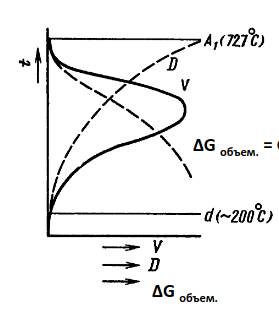
\includegraphics[width=0.6\textwidth]{perlite_speed.png}\caption{Зависимость скорости перлитного превращения (сплошная линия) от температуры}\label{fig:perlite_speed}
\end{figure}
\par Кинетика перлитного превращения описывается уравнение Колмогорова-Аврами (JMAK):
\begin{equation}
y=1-e^{-kt^n}
\label{eq:JMAK}  
\end{equation}
Здесь y - степень превращения, t - время, n - эмпирический параметр.
\begin{figure}[h!]
\centering
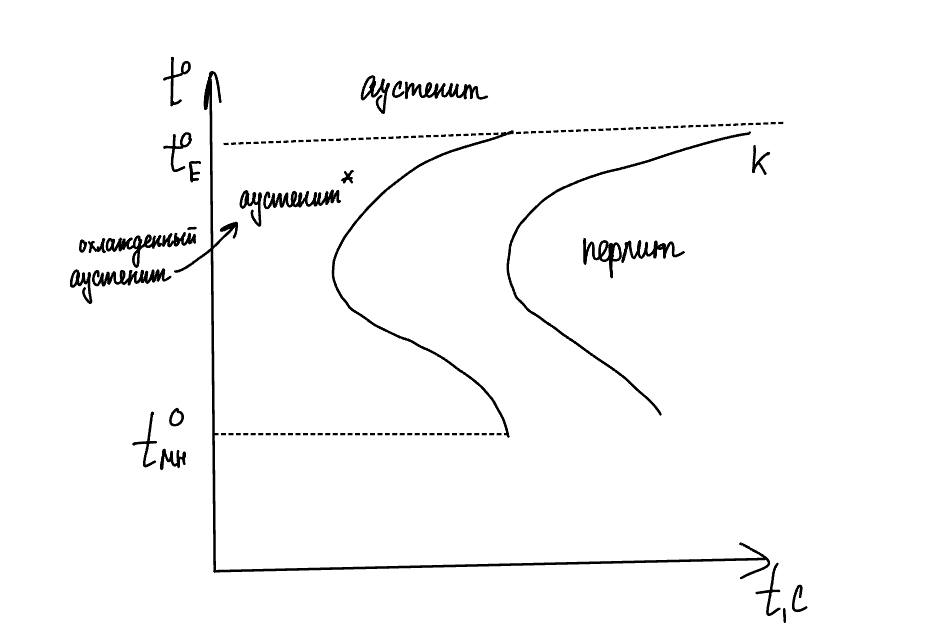
\includegraphics[width=0.4\textwidth]{TTT-diagram.png}\caption{Общий вид ТТТ-диаграммы}\label{fig:TTT-diagram}
\end{figure}
\par Для описания фазовых превращений часто используют изотермические ТТТ-диаграммы (time-transformation-temperature), выглядящие следующим образом (рис. \ref{fig:TTT-diagram}). На рисунке использованы следующие обозначения: н - кривая начала перлитного превращения, к - кривая завершения перлитного превращения, $t_{\text{МП}}^\circ$ - температура начала мартенситного перехода. 
\par На ТТТ-диаграммах удобно выбирать режимы термообработки. Если кривая охлаждения не заходит в перлитную область, то осуществляется закалка на мартенсит. Дифференцировка перлита (перлит, сорбит, троостит - $\lambda \downarrow$) зависит от профиля охлаждения (рис. \ref{fig:cooling_profile}).
\begin{figure}[h!]
\centering
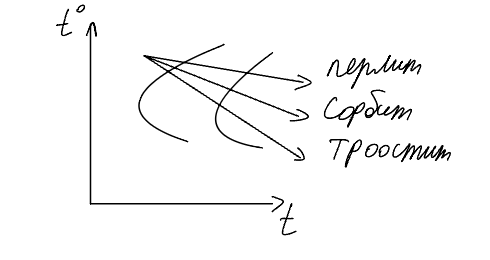
\includegraphics[width=0.4\textwidth]{cooling_profile.png}\caption{Дифференцировка перлита и профиль охлаждения}\label{fig:cooling_profile}
\end{figure}
По ТТТ-диаграммам удобно иллюстрировать различные виды отжига 2-го рода (рис. \ref{fig:annealing2_types}).
\begin{figure}[h!]
\centering
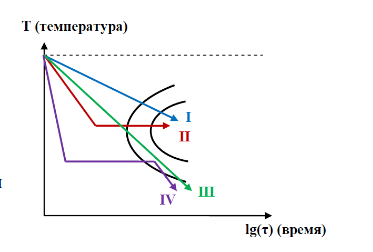
\includegraphics[width=0.4\textwidth]{annealing2_types.png}\caption{Основные виды отжига 2-го рода}\label{fig:annealing2_types}
\end{figure}
На рисунке \ref{fig:annealing2_types} 1 - полный отжиг (медленно, в грубый перлит), 2 - изотермический отжиг (в грубый перлит), 3 - нормализация (в сорбит), 4 - патентирование (в троостит). \par\textit{ИМХО, автор рисунка ошибся с 3 и 4. Кривые следует аккуратно заканчивать в перлитной области, а то это уже не троосит с сорбитом, а бейнит какой-то}